\section*{{ADDERS}}

An adder is a digital logic circuit in electronices that implement the addition of numbers.
Half adder: is a combinational circuit that performs the addition of two bits, this circuit needs two binary inputs and two binary outputs.
Adding two single-bit binary values, X and Y produces a sum S bit and a carryout C-out bit.





\textbf{TABLE 3: Input and Output for the Half Adder}

\[
\begin{array}{|c|c||c|c|}
\hline
\multicolumn{2}{|c||}{\textbf{Input}} & \multicolumn{2}{c|}{\textbf{Output}} \\
\hline
x & y & s & c \\
\hline
1 & 1 & 0 & 1 \\
\hline
1 & 0 & 1 & 0 \\
\hline
0 & 1 & 1 & 0 \\
\hline
0 & 0 & 0 & 0 \\
\hline
\end{array}
\]

\vspace{0.5cm}



\begin{figure}[H]
    \centering
    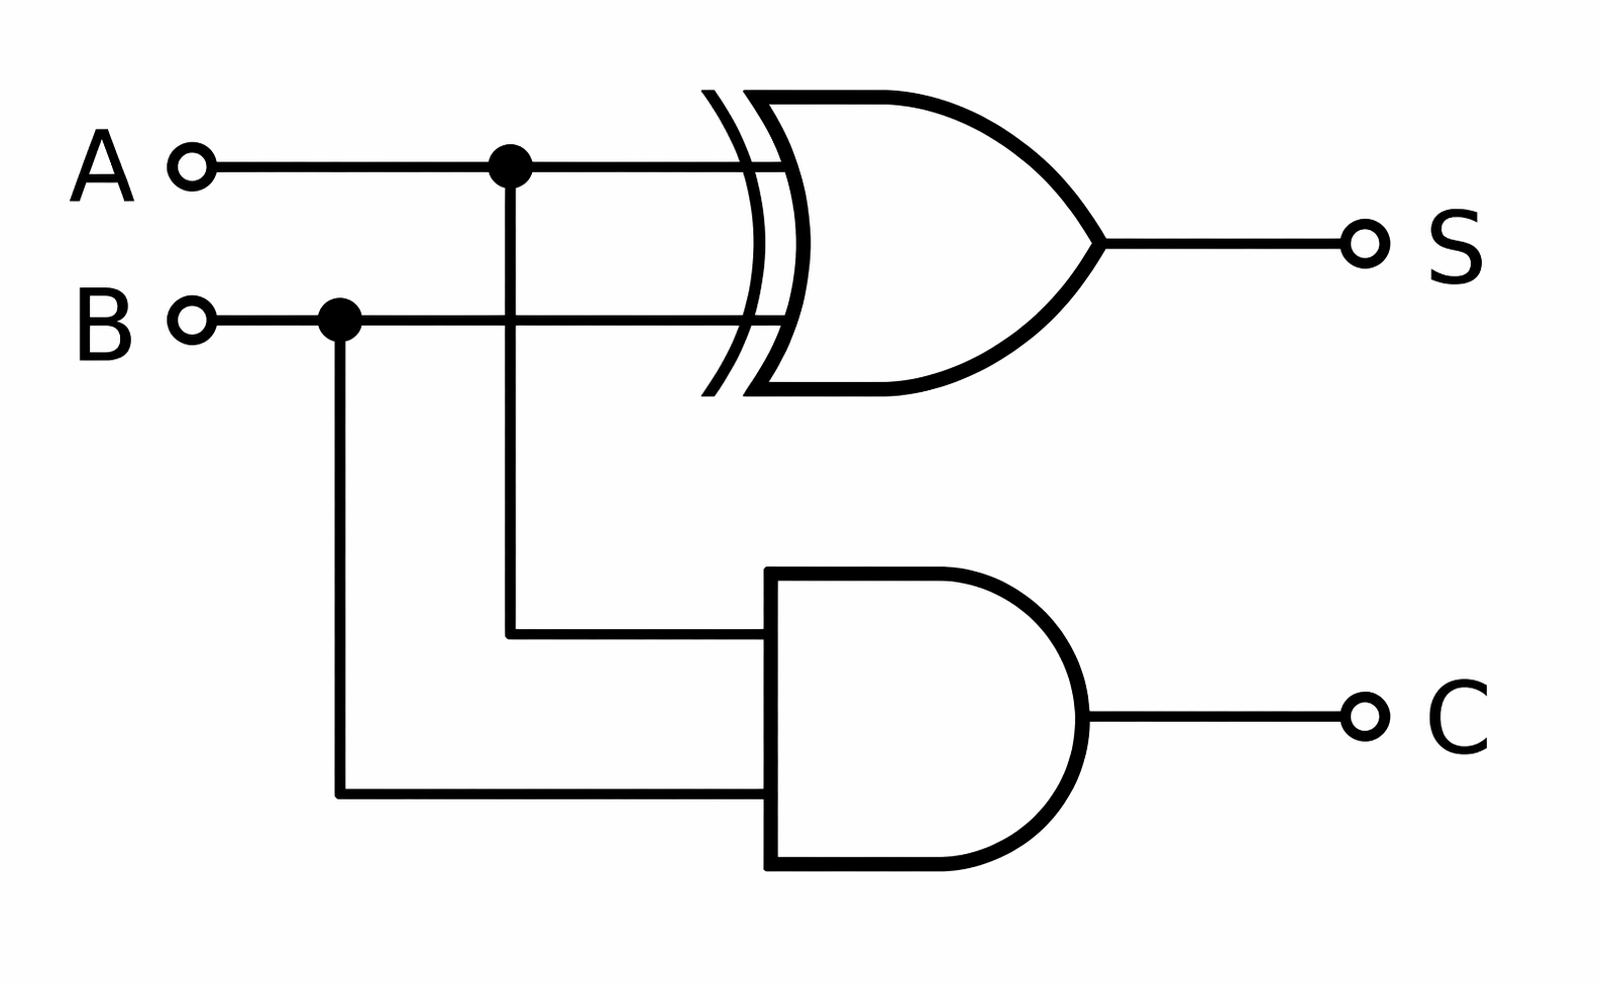
\includegraphics[width=0.6\textwidth]{images/image.png}
    \caption{FIGURE 7: The Half Adder}
    \label{fig:half_adder}
\end{figure}


\section* {Full Adder}

A full adder is a combinational circuit that performs the addition of three bits (two significant bits and a previous carry).
.it consists of three outputs and two outputs, where two inputs are the bits to be added , the third input represent the carry from the previous position.
. Adding two single-bit binary values Xand Y with a carry input bit C-in produces a sum bit Sand a carry out C-out bit.

 The Boolean expressions for the full adder are
\[
s = xyc_i + x\bar{y}\bar{c_i} + \bar{x}y\bar{c_i} + \bar{x}\bar{y}c_i
\]
and
\[
c_{i+1} = xyc_i + xy\bar{c_i} + x\bar{y}c_i + \bar{x}yc_i.
\]
These expressions account for all possible combinations of the three inputs and ensure that the correct sum and carry values are produced. The full adder is more powerful than the half adder because it allows the inclusion of carry propagation, which is essential for performing addition on numbers with more than one bit.

\begin{center}
\textbf{{TABLE 4}}\\[0.2cm]
\textbf{Input and Output for the Full Adder}
\[
\begin{array}{|c|c|c||c|c|}
\hline
\multicolumn{3}{|c||}{\textbf{Input}} & \multicolumn{2}{c|}{\textbf{Output}}\\
\hline
x & y & c_i & s & c_{i+1} \\
\hline
0 & 0 & 0 & 0 & 0 \\
\hline
0 & 0 & 1 & 1 & 0 \\
\hline
0 & 1 & 0 & 1 & 0 \\
\hline
0 & 1 & 1 & 0 & 1 \\
\hline
1 & 0 & 0 & 1 & 0 \\
\hline
1 & 0 & 1 & 0 & 1 \\
\hline
1 & 1 & 0 & 0 & 1 \\
\hline
1 & 1 & 1 & 1 & 1 \\
\hline
\end{array}
\]
\end{center}


\begin{figure}[H]
    \centering
    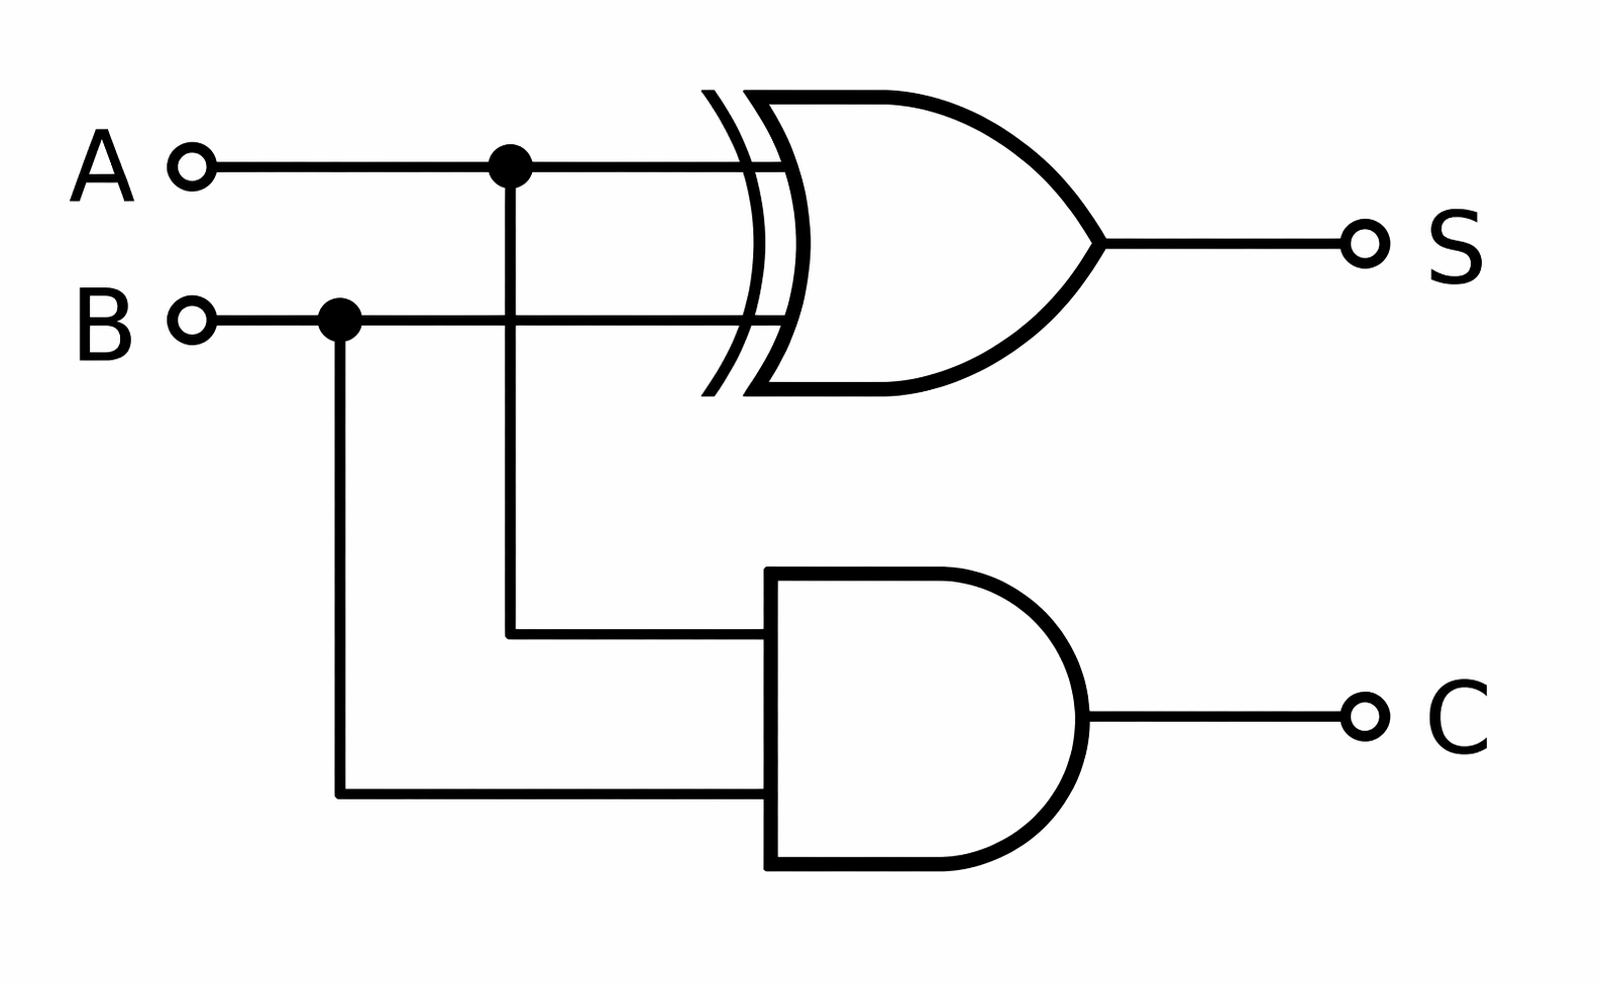
\includegraphics[width=0.7\textwidth]{images/image.png}
    \caption{FIGURE 8: The Full Adder}
    \label{fig:full_adder}
\end{figure}


\section{EXCERCISES}

\textbf{1.} Design a circuit that implements majority voting for five individuals.

\vspace{0.3cm}

\textbf{2.} Design a circuit for a light fixture controlled by four switches, where flipping one of the switches turns the light on when it is off and turns it off when it is on.

\vspace{0.3cm}

\textbf{3.} Show how the sum of two five-bit integers can be found using full and half adders.

\vspace{0.3cm}





\textbf{4.} Construct a circuit that compares the two-bit integers $(x_1x_0)_2$ and $(y_1y_0)_2$, returning an output of 1 when the first of these numbers is larger and an output of 0 otherwise.

\vspace{0.3cm}

